Over the years, Google has been building its own distinctively designed data
centers, deploying numerous machines around the world. Within these facilities,
arrays of servers operate continuously, fueling essential services that a
multitude of people rely on daily. Nevertheless, the process of designing data
centers is a complex optimization challenge with multiple factors to consider.
While the primary objective is to optimize the utilization of computing capacity
offered to users, it is equally imperative to ensure the uninterrupted provision
of computing power, even in scenarios where hardware failures are inevitable.
Drawing inspiration from these engineering challenges, this problem presents a
Google Data Center design scenario that closely mirrors real-world complexities,
as we describe next.

The data center, as outlined in the problem statement, is modelled as collection
of distinct~\textit{rows}. Each row consists of a specific number of available
spaces referred to as~\textquote{slots}, designated for the placement of
servers.~Notably, this number of slots remains consistent across all rows within
the data center.~Additionally, certain slots within the data center may be
unusable due to other installations that impose restrictions on the utilization
of those specific spaces. However, because rows share resources, such as
electrical power, a hardware failure in one row can render the entire row of
servers inaccessible.

In~\Cref{fig:data-center-layout}, an illustration depicts a layout featuring two
rows, each consisting of a total of seven slots. Note that some of these slots
are marked as unavailable, as indicated by the cross symbol.

\begin{figure}[h]
  \centering
  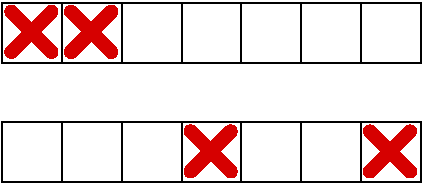
\includegraphics[width=0.6\textwidth,keepaspectratio]{../assets/dc/dc-rows-no-labels.pdf}
  \caption{Example Data Center Layout}
  \label{fig:data-center-layout}
\end{figure}

The servers are defined by a tuple that includes two attributes: the
\textit{size} of the server, which is measured in terms of the number of
consecutive slots occupied by the machine, and the computing~\textit{capacity}
of the server, represented as an integer value that indicates the machine's CPU
resources.~The~\Cref{tab:dc-example-properties} presents potential values for
these parameters, showcasing examples of four distinct servers.

\begin{table}[ht]
  \centering
  \begin{tabular}{ccc}
  \toprule Server & Size &
  Capacity                    \\ \midrule
  1               & 3    & 2  \\
  2               & 2    & 5  \\
  3               & 3    & 10 \\
  4               & 2    & 3  \\
  \bottomrule
\end{tabular}
  \caption{Server Properties}
  \label{tab:dc-example-properties}
\end{table}

Moreover, when servers are positioned within the data center rows, they are
logically associated with resource~\textit{pools}, to which they can contribute
their individual computing capacities.~The capacity of a pool is defined as the
collective sum of the capacities of all the servers allocated to it.

For clarification,~\Cref{fig:data-center-layout-with-servers} offers a potential
assignment of servers based on the data center layout depicted in
~\Cref{fig:data-center-layout}, and the server attributes provided
in~\Cref{tab:dc-example-properties}. In this particular case, servers are
allocated to two distinct resource pools.

\begin{figure}[h]
  \centering
  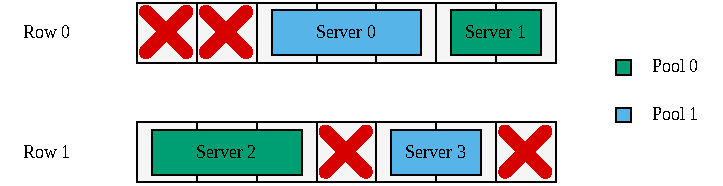
\includegraphics[width=0.9\textwidth,keepaspectratio]{../assets/dc/dc-example.pdf}
  \caption{Example Server Assignment}
  \label{fig:data-center-layout-with-servers}
\end{figure}

Upon closer examination of the this example, we can deduce that ensuring the
reliability of a specific resource pool implies the distribution of servers
across various rows. This approach ensures that in the event of a row failure,
the pool can still operate with diminished capacity, drawing upon the servers
located in the unaffected rows.~In the context of the problem, this represents
the concept of a~\textit{guaranteed capacity} for a pool, which can be defined
as follows:

Let $\mathcal{P}$ be the number of resource pools, the guaranteed capacity
($gc_{p}$) of a given pool ($p = 1, \ldots, \mathcal{P}$), is a measure of the
remaining computing capacity available in the event that at most one arbitrary
row~($r = 1, \ldots, \mathcal{R}$) of the data center becomes inoperable.
Formally, this can be described as shown in~\Cref{eq:guaranteed-capacity}, where
$\mathcal{M}$ denotes the number of servers available, $c_{m}$ the computing
capacity of a given server ($m = 1, \ldots, \mathcal{M}$), and $x_{m,p,r}$ is a
binary variable indicating whether the server $m$ is present (1) or absent
(0) in pool $p$ for row $r$.

\begin{equation}
  \label{eq:guaranteed-capacity}
  {gc}_{p} = \min_{r = 1}^{\mathcal{R}} \left({\sum_{m = 1}^{\mathcal{M}}{\sum_{i = 1}^{\mathcal{R}} c_{m} \cdot x_{m,p,i}}} - {\sum_{m = 1}^{\mathcal{M}} c_{m} \cdot x_{m,p,r}}\right)
\end{equation}

The objective of this problem can thus be succinctly defined as follows: given a
layout description of a data center, the goal is to determine the optimal
arrangement of servers within the data center rows and assignment of these
servers to resource pools, such that, the minimum guaranteed capacity across all
pools is maximized. Mathematically, this can be expressed as shown
in~\Cref{eq:objective}.

\begin{equation}
  \label{eq:objective}
  \max{f(s)} = \min_{p = 1}^{\mathcal{P}}{{gc}_{p}}
\end{equation}

To clarify all the concepts discussed the~\Cref{ex:problem-scoring} demonstrates
how the objective is evaluated for the allocation of servers presented
in~\Cref{fig:data-center-layout-with-servers}.

\begin{example}[Objective Evaluation]
  \label{ex:problem-scoring}
  Consider the capacities assigned to each resource pool per row, as illustrated
  in~\Cref{tab:dc-gc-example}.

  \begin{table}[ht]
    \centering
    \begin{tabular}{@{\extracolsep{4pt}}cccccc@{\extracolsep{4pt}}}
  \toprule
  Pool & Row 1 & Row 2 & Guaranteed Capacity & \textbf{$f(x)$}              \\ \midrule
  1    & 5     & 10    & 5                   &                              \\
  2    & 2     & 3     & 2                   & \multirow{-2}{*}{\textbf{2}} \\
  \bottomrule
\end{tabular}
    \caption{Guaranteed Capacity \& Score}
    \label{tab:dc-gc-example}
  \end{table}

  The score obtained for this server placement, as determined by the evaluation
  of the objective~\ref{eq:objective}, is calculated as $\min(5, 2) = 2$.
\end{example}

To conclude, several constraints are imposed on various parameters that
describe the data center design for this problem. These constraints are as
follows:

\begin{description}
  \item[\textbf{$\mathcal{R}$.}] The number of rows in the data center~($ 1 \leq \mathcal{R} \leq 1000$)
  \item[\textbf{$\mathcal{S}$.}] The number of slots in each row of the data center~($ 1 \leq \mathcal{S} \leq 1000$)
  \item[\textbf{$\mathcal{U}$.}] The number of unavailable slots~($ 0 \leq \mathcal{U} \leq \mathcal{R} \times \mathcal{S}$)
  \item[\textbf{$\mathcal{P}$.}] The number of resource pools~($ 1 \leq \mathcal{P} \leq 1000$)
  \item[\textbf{$\mathcal{M}$.}] The number of servers to be allocated~($ 1 \leq \mathcal{M} \leq \mathcal{R} \times \mathcal{S}$)
\end{description}